\documentclass[conference]{IEEEtran}

%\usepackage[russian]{babel}
\usepackage[justification=centering]{caption}
\usepackage[backend=bibtex]{biblatex}
\usepackage{fontspec}
\usepackage[final]{graphicx}
\usepackage{float}
\usepackage{subcaption}
\usepackage{listings}
\usepackage{array}
\usepackage{xcolor}
\usepackage{graphicx}
\usepackage{tikz}
\usepackage{pgfplots}
%\usepackage{geometry}
\graphicspath{{./images/}}

\setmainfont{Spectral Light}%{Times New Roman}

\definecolor{codegreen}{rgb}{0,0.6,0}
\definecolor{codegray}{rgb}{0.5,0.5,0.5}
\definecolor{codepurple}{rgb}{0.58,0,0.82}
\definecolor{backcolour}{rgb}{0.95,0.95,0.92}

\lstdefinestyle{mystyle}{
    backgroundcolor=\color{white},   
    commentstyle=\color{codegreen},
    keywordstyle=\color{magenta},
    numberstyle=\color{codegray},
    stringstyle=\color{codepurple},
    basicstyle=\ttfamily\footnotesize,
    morekeywords={*,procedure, if, rol, cmpj, setmask, then, else, endif, cmpjn, is, not, and, return},            % if you want to add more keywords to the set
    breakatwhitespace=false,         
    breaklines=true,                 
    captionpos=b,                    
    keepspaces=true,                 
    numbers=left,                    
    numbersep=10pt,
    xleftmargin=7mm,
    xrightmargin=0mm,
    showspaces=false,                
    showstringspaces=false,
    showtabs=false,                  
    tabsize=4
}
\lstset{style=mystyle}
\lstset{linewidth=9cm}
\bibliography{monetec} 


\begin{document}
\author{
    \IEEEauthorblockN{Nikita Nikiforov}
    \IEEEauthorblockA{\textit{Lomonosov Moscow State University}\\
    Moscow, Russia\\
    nickiforov.nik@gmail.com}
    \and
    \IEEEauthorblockN{Yulia Skobtsova}
    \IEEEauthorblockA{\textit{Lomonosov Moscow State University}\\
    Moscow, Russia\\
    xenerizes@lvk.cs.msu.ru}
    \and
    \IEEEauthorblockN{Dmitry Volkanov}
    \IEEEauthorblockA{\textit{Lomonosov Moscow State University}\\
    Moscow, Russia\\
    volkanov@asvk.cs.msu.ru}
    }
\title{
    Data Structures for Classification in the Network Processor without the Separated Associative Device
}
\maketitle
    \begin{abstract}
        This paper addresses the problem of packet classification within a network processor (NP) architecture 
        without the separate associative device.
        By the classification, we mean the process of identifying a packet by the header.
        The classification stage requires the implementation of data structures to store the classification tables.
        In our work we consider NP without the associative memory.
        To classify the packets in such an NP, we propose to use search trees.
        The reason for choosing these structures were the limitations of the NP.
        We propose use of an AVL tree, path-compressed trie and binary one bit tree.
        An evaluation of the implemented data structures was performed on a 
        simulation model of the NP.
        Evaluation of the adapted AVL tree showed that it allowed reducing 
        the number of network processor cycles for processing one packet and reducing the use of memory of the pipeline's computing blocks.
    \end{abstract}
    
    \begin{IEEEkeywords}
        Network processor, software-defined networks, packet classification, search trees.
    \end{IEEEkeywords}
    
    \section{Introduction}
        At present, software-defined networks (SDN)~\cite{smel2012open} are in active developing
        and require high-performance switches~\cite{bifulco2018survey}. 
        The main functional element of the high-perfomance SDN switch is a programmable network processor.
        The network processor (NP) is a System-On-Chip specialized for the network packet processing~\cite{chao2007high:1}.
        Programmable NP is an NP such that support to
        change the packet processing program and set of distinguishable
        header fields. Then, you can switch to new protocols stack~\cite{bezzubtsev2019ob-odnom183708319}.

        This article will discuss the packet classification.
        The classification is the process of identification of a network packet 
        by its header fields.
        The classification table is a set of rules, containing the match fields, 
        by which the packet is identified,
        and the actions that the NP performs on this packet.
        Match field is represented in NP as a bit string. 
        Bit string can match exactly or by the longest prefix.
        Thus, to perform the classification, the NP must include an associative device. 
		Associative memory is commonly used to implement this device.
        However, a single associative memory controller will be the bottleneck, 
        since it must be available for all stages of the packet processing pipeline.
        In our work, we propose data structures for searching in classification 
        tables by single match field in the NP without a separated associative device.
    \section{Network processor architecture}
        \label{section:problem}
        In considered NP the pipeline architecture is used, each pipeline consists of 10 computing blocks. 
        To avoid complex organization of memory, there is no associative memory in the considered NP. 
        The NP uses the same memory for commands and data.
         
        Let consider the pipeline NP architecture. 
        Each computing block has access to the memory area where the program with data are located.
        There is a limit on the number of clock cycles that one packet can process on a processing block, 
        it corresponds to 25 clock cycles.
        All memory to store classification table is 2 megabytes.
        Due to the instruction set architecrute, there is no separate memory area where data is stored. 
        Therefore, the microcode contains all the data, required to classify packets.

    \section{Proposed data structures}
        Let consider the proposed data structures.
        \subsection{Binary one bit tree}
            The most common~\cite{behdadfar2009scalar} data structure for searching by 
            the longest-prefix match is a binary one bit tree~\cite{chao2007high:1}.
            The tree is built according to the given prefixes such that each bit of the prefix has its own tree node in the tree. 
            The search is performed by the bits of the bit string for which the search is performed. 
            The search ends when the empty vertex is reached, the search result is the last viewed prefix.
 
        \subsection{Path-compressed trie}
            The optimization of the binary one bit tree~\cite{ruiz2001survey} is a path-compressed trie. 
            To build this tree you must build a binary one bit tree, 
            then perform a compression procedure. All the vertices that have only one sheet, 
            are reduced, and the number of missed nodes is recorded at the next node. 
            To use path-compressed trie, a procedure for node construction was develop.
        \subsection{AVL tree}
            AVL tree is balancing tree. 
            Only scalar values can be stored in this tree nodes.
            The AVL tree use an algorithm for presenting prefixes like scalar values.
            Representing prefixes as scalar prefixes allows using a larger set of data structures~\cite{behdadfar2009scalar}. 

                Algorithm for representing prefixes as scalar values 
                is necessary to save and search for prefixes in the AVL tree. 
                The algorithm allows comparing prefixes with each other~\cite{behdadfar2011coded}:
                \begin{itemize}
                    \item If the lengths of the two prefixes match, they are compared as two scalar values.
                    \item If the length of the $q$ prefix is smaller than the length of the $p$ prefix, 
                        the first $len(q) - 1$ bits of both prefixes are compared as scalar values.
                \end{itemize}
    
    \section{Evaluation}
        Evaluation was conducted on a simulation model of the NP. 
        To compare data structures, the following parameters were considered: 
        the number of clock cycles per packet processing, program size.
        Developed data structures were evaluated for different size classification tables:
        1000, 8000, 16000, 32000, 64000 bit rows. Bit rows of different lengths will be used:
        32, 48 bits. For each data structure, studies will be carried out with traffic 
        covering the loaded table into a simulated network processor model.
        \\
            \begin{figure}
                \centering
                \subfloat[Bit string length]{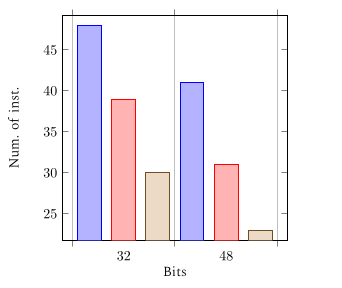
\includegraphics[width=0.5\linewidth]{Bits.png}}
                \subfloat[Program size]{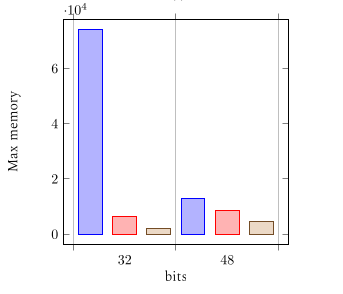
\includegraphics[width=0.5\linewidth]{Memory.png}}
                \caption{Data structures comparison.}
                \label{graph:all}
            \end{figure}
            \\
            Figure.~\ref{graph:all} shows the comparison of 
            implemented data structures by the average number of instructions per one packet and
            by the program size.
            You can see that the AVL tree shows the best result of all the implemented data structures.
            
            For the AVL tree the maximum memory size occupied 
            by the data structure does not exceed 2 MB and the average amount of
            instructions for classifying one packet is 30 and 23 for 32-bit and 48-bit bit strings respectively.
            For the path-compressed trie, the maximum amount of memory occupied 
            by the data structure does not exceed 8.5 MB, and the average number of
            instructions for classifying one packet is 39 and 31 for 32-bit and 48-bit bit strings respectively.

    \section{Conclusion}
        In this paper the problem of classifying packets in the considered architecture of the NP was considered.
        Data structures have been developed to classify packets by one packet header field
        in the NP without separated associative memory.
        Developed data structures were evaluated on the NP simulation model.
        It was concluded from the data obtained during the evaluation that only the AVL tree satisfies the limitations of NP.

        As a direction for further research, we can indicate for further optimization of implemented data structures,
        to reduce the amount of memory occupied by data structures, as well as to consider changes in the NP architecture.

\printbibliography{}
\end{document}
